\chapter{Simulation Study Supplementary material}
\label{chap:AppendixB}
The framing of the simulated PET protocols are given in table~\ref{table:FrameTimings}. The TACs used in simulations were made using using equation~\ref{2TCM}.
A selection of the simulated kinetic parameters is given in table~\ref{table:KineticValues} and the corresponding TACs are shown in figure~\ref{fig:zubal_phantom}.

\begin{table}[htb!]
\caption{Framing of simulated DWB protocols (sec). Frames used for Patlak analysis in bold.}
\label{table:FrameTimings}
%\begin{center}
\begin{tabular}{|c|c|c|c|c|c|c|c|c|c|c|}
\toprule
    \multicolumn{1}{c}{} &\multicolumn{2}{c}{Single Bed} &  \multicolumn{2}{c}{DWB-1} &  \multicolumn{2}{c}{DWB-2} &    \multicolumn{2}{c}{DWB-3} & \multicolumn{2}{c}{DWB-4}   \\
    \midrule
   {Frame number}& start&duration& start&duration & start&duration & start&duration & start&duration \\
\midrule
1  & 0    & 20  & 206  & 20   & 205  & 20   & 205  & 20  & 0    & 20 \\
2  & 20   & 20  & 366  & 20   & 327  & 20   & 355  & 20  & 20   & 20 \\
3  & 40   & 20  & 536  & 30   & 461  & 30   & 437  & 30  & 40   & 20 \\
4  & 60   & 20  & 776  & 60   & 676  & 60   & 662  & 30  & 60   & 20 \\
5  & 80   & 30  & \textbf{1136} & \textbf{60}   & \textbf{1018} & \textbf{60}   & 805 & 60   & 80   & 20 \\
6  & 110  & 30  & \textbf{1568} & \textbf{132}  & \textbf{1360} & \textbf{60}   & \textbf{1255} & \textbf{60}   & 100  & 20 \\
7  & 140  & 30  & \textbf{2288} & \textbf{132}  & \textbf{1772} & \textbf{116}  & \textbf{1465} & \textbf{60}   & 120  & 20 \\
8  & 170  & 60  & \textbf{3008} & \textbf{132}  & \textbf{2422} & \textbf{116}  & \textbf{1915} & \textbf{60}   & 140  & 20 \\
9  & 230  & 60  & & & \textbf{3072} & \textbf{116}  & \textbf{2195} & \textbf{116}  & 160  & 20 \\
10 & 290  & 60  & & & & & \textbf{3065} & \textbf{116} & 206  & 20 \\
11 & 350  & 60  & &  &  &  &  &  & 366  & 20 \\
12 & 410  & 60  & &  &  &  &  &  & 536  & 30 \\
13 & 470  & 120 & &  &  &  &  &  & 776  & 60 \\
14 & 590  & 120 & &  &  &  &  &  & \textbf{1136} & \textbf{60}  \\
15 & 710  & 120 & &  &  &  &  &  & \textbf{1568} & \textbf{132} \\
16 & 830  & 300 & &  &  &  &  &  & \textbf{2288} & \textbf{132} \\
17 & \textbf{1130} & \textbf{300} & &  &  &  &  &  & \textbf{3008} & \textbf{132} \\
18 & \textbf{1430} & \textbf{300} & & & & & & & & \\
19 & \textbf{1730} & \textbf{300} & & & & & & & & \\
20 & \textbf{2030} & \textbf{300} & & & & & & & & \\
21 & \textbf{2330} & \textbf{300} & & & & & & & & \\
22 & \textbf{2630} & \textbf{300} & & & & & & & & \\
23 & \textbf{2930} & \textbf{300} & & & & & & & & \\
24 & \textbf{3230} & \textbf{300} & & & & & & & & \\
\toprule
\end{tabular}
%\end{center}
\label{tab:multicol}
\end{table}

\begin{table}[htb!]
\caption{Parameters of simulated 2 tissue compartment models in the zubal brain phantom.}
\label{table:KineticValues}
%\begin{center}
 \begin{tabular}{c c c c c c c c} 
\toprule
 Region & $K_1 (ml \cdot g^{-1} \cdot min^{-1})$ & $k_2 (min^{-1})$ & $k_3 (min^{-1})$ & $V_b$ & $K_i (min^{-1})$ & Patlak slope(SB) \\ [0.5ex] 
\midrule
%\textbf{Bones}       & 0.0027 & 0.0033   & 0.001 & 0        & 0.0006 & 0.0023 \\
\textbf{White}       & 0.047  & 0.07     & 0.035 & 0.03     & 0.0157 & 0.0149 \\
\textbf{Cortex}      & 0.102  & 0.073    & 0.049 & 0.03     & 0.0410 & 0.0390 \\
\textbf{Cerebellum}  & 0.07   & 0.07     & 0.04  & 0.03     & 0.0255 & 0.0242 \\
\textbf{Putamen}     & 0.081  & 0.052    & 0.032 & 0.03     & 0.0309 & 0.0302 \\
\textbf{Caudate}     & 0.081  & 0.052    & 0.032 & 0.03     & 0.0309 & 0.0302 \\
\textbf{Thalamus}    & 0.092  & 0.052    & 0.026 & 0.03     & 0.0307 & 0.0305 \\
\textbf{Muscle}      & 0.05   & 0.163177 & 0.03  & 0.25     & 0.0078 & 0.0055 \\
\toprule
\end{tabular}
%\end{center}
\label{tab:multicol2}
\end{table}

\begin{equation} \label{2TCM}
{C_{PET}}(t) = (1-V_B)\Big({\frac{K_1 k_2}{k_2+k_3}} e^{-(k_2+k_3)t} + {\frac{K_1 k_3}{k_2+k_3}}\Big)  C_{P}(t) + V_B C_{P}(t) \ \ \ \
\end{equation}

\begin{figure} [ht!]
\centering
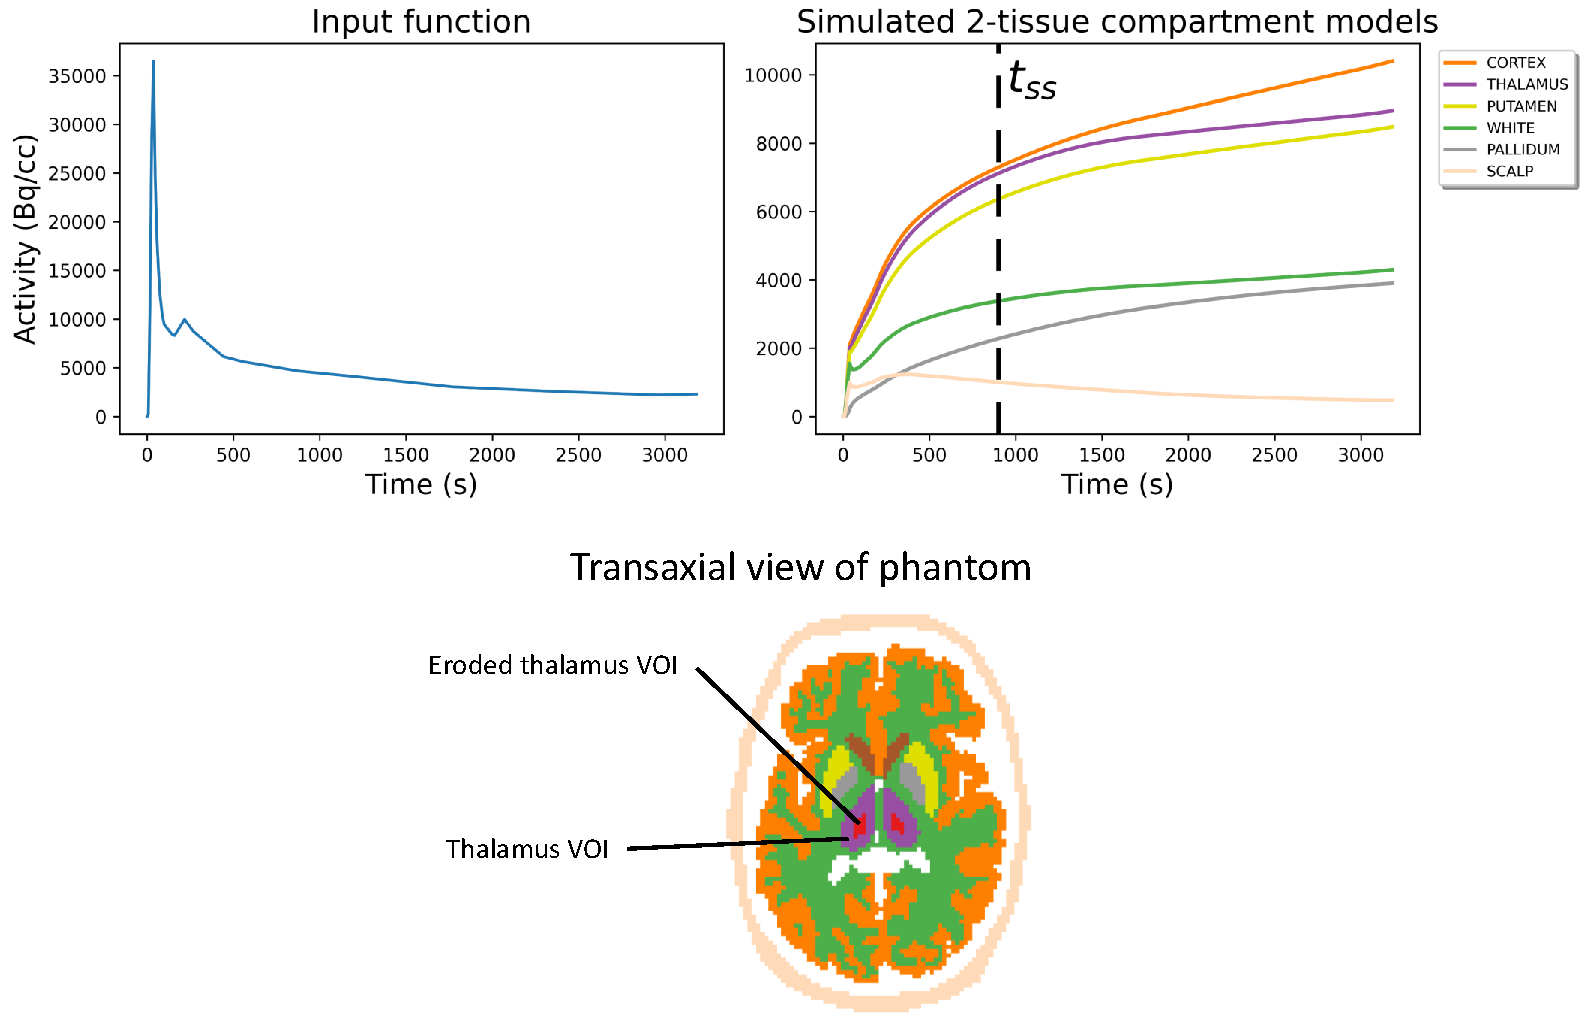
\includegraphics[width=140mm ,angle=0]{appendices/figures/phantom_TACs.pdf}
\caption{Input function and selection of simulated 2-tissue compartment model TACs (top), and transaxial view of the segmented zubal phantom, with the addition of an eroded thalamus VOI (bottom). The same colours are used for the TACs and the VOIs.} 
\label{fig:zubal_phantom}
\end{figure}


\begin{table}[h!]
\centering
\caption{\label{tab:VOIs}VOIs used for evaluation.}
\begin{tabular}{llll}
\toprule
\textbf{VOI Name} & \textbf{Number of voxels} & \textbf{Volume ($cm^3$)}  \\
\midrule
Thalamus        & 915   & 12.40      \\
Eroded thalamus & 218   & 2.95       \\
Cortex          & 46588 & 631.36     \\
\toprule
\end{tabular}
\end{table}


